\documentclass[12pt]{article}

% Packages
\usepackage[margin=1in]{geometry}
\usepackage{setspace}
\usepackage{graphicx}
\usepackage{amsmath, amssymb}
\usepackage{hyperref}
\usepackage{titlesec}
\usepackage{mdframed}
\usepackage{xcolor}
\usepackage{float}


% Spacing
\setstretch{1.2}

\usepackage{xcolor}
\usepackage{hyperref}

\hypersetup{
    colorlinks=true,
    linkcolor=blue,
    urlcolor=blue,
    citecolor=blue
}

\let\oldhref\href
\renewcommand{\href}[2]{\oldhref{#1}{\underline{#2}}}

% Section formatting
\titleformat{\section}{\large\bfseries}{\thesection}{1em}{}
\titleformat{\subsection}{\normalsize\bfseries}{\thesubsection}{1em}{}

% Title info
\title{\textbf{Voter FAQ Source Classification}}
\author{Madison Byrd \\
Building Secure Software \\
}
\date{\today}

\begin{document}

\maketitle
\newpage

\section{Report}

In this project I trained two models to guess if an FAQ source for voters was a primary or secondary source,
and used LIME to investigate why the model made its decision. 75\% of data was used for training and 
25\% was used for testing. 

The results are included in this GitHub repository. The model considered the words "purposes", "voter",
and "Iowa" to be strong indicators of a primary source, and "ID", "available", and "hours" to be
strong indications of a secondary source, with "ID" being exceptionally strong. An example is as follows:

\begin{figure}[H]
    \centering
    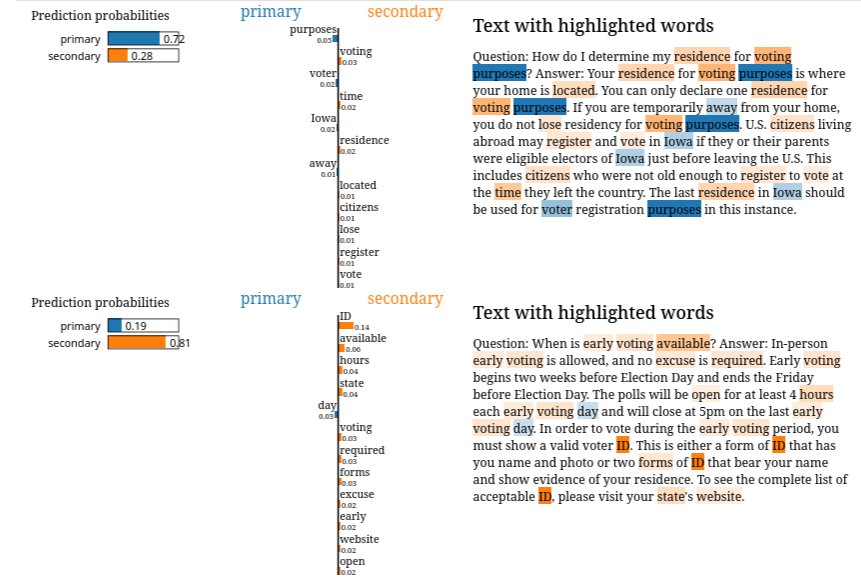
\includegraphics[width=1\textwidth]{analysis.png}
    \caption{Examples of primary and secondary guesses by the model and their reasoning}
\end{figure}


These models seem shockingly good at guessing (the logistic regression got an F1 score of 0.88 and 
an ROC AUC score of 0.96 while Multinomial Naive Bayes scored 0.86 and 0.95 respectively). 
I would be interested to see how it performs on different data, because this data seems to be 
very speciifc to certain documents from Iowan elections.

\end{document}
